\documentclass{article}
\usepackage[utf8]{inputenc}
\usepackage{kotex}
\usepackage{color}
\usepackage[T1]{fontenc}
\usepackage{graphicx}
\usepackage{subfigure}
\usepackage{caption}
\usepackage{float}
\title{HW0}
\author{B711028 김영민}
\date{2021/9/10}


\begin{document}
	
	\maketitle
	
\section{자기소개}

	저는 홍익대학교 컴퓨터공학과 17학번 김영민입니다. 이번 송하윤 교수님의 자료구조 수업을 들음으로써 자료 정렬, 그래프 그리기 등 자료의 정리에 관해 잘 배우고 싶습니다. 자료구조의 알고리즘과 여러 수학의 공식들을 익히고 이것을 실제 코딩에 접목함으로써 저의 코딩 실력과 알고리즘을 짜는 실력을 동시에 향상 시키고 싶습니다. C++은 그래도 많이 사용을 해봐서 이 수업을 배우기 전에는 단순한 반복문과 조건문을 사용하는 것에만 익숙하였는데, 이 수업을 배우고 난 후에는 재귀 반복문과 포인터의 활용, template 함수의 활용을 잘 해내는 능력을 키우고 싶습니다. 1장을 나갈때 교수님께서 재귀 반복문에 대해 설명을 하셨는데, 확실히 재귀 반복문이 그냥 일반적인 반복문보다 시간, 공간적 측면에서 좀 더 효과적인 것 같습니다. 이런 부족한 면을 이번 자료구조 수업을 들음으로써 좀 더 코딩 실력을 키우고 싶습니다.
	\vspace{2em}	
\section{수식작성}
	\colorbox{black}{\textcolor{white}{\#31}}  \underline{\textbf{등차수열의 합}}\newline
◈ $ S_n $
\vspace{0.1em}
\setlength{\parindent}{2ex}\par

- 첫째항부터 제$n$항까지의 합\newline
◈  첫째항이 $ a_1 $, 제$n$항이 $ a_n $인

\setlength{\parindent}{3ex}\par 등차수열 $\{ a_n\} $의 합 $ S_n $
\setlength{\parindent}{2ex}\par\vspace{0.1em}
- $S_n  = \frac{n(a_1 + a_n)}{2} $\newline
◈  첫째항이 $ a_1 $, 공차가 $ d $인

\setlength{\parindent}{3ex}\par 등차수열 $\{a_n\}$의 합 $S_n$
\setlength{\parindent}{2ex}\par\vspace{0.1em}
- $S_n  = \frac{n\{2a_1 + (n-1)d\}}{2} $\newline
◈  일반항 $a_n$과 합 $S_n$ 사이의 관계
\setlength{\parindent}{2ex}\par
- 수열 $\{a_n\}$의 첫째항부터
\setlength{\parindent}{3ex}\par
제 $n$항까지의 합을 $S_n$이라고 하면
\setlength{\parindent}{3ex}\par
$a_n = S_n - S_{n-1}(n\geq2)$
\setlength{\parindent}{3ex}\par
$a_1 = S_1$
\vspace{2em}
\section{가장 좋아하는 그림}
\begin{figure}[H]
\begin{center}
		
\includegraphics{Hongik.jpg}	
		\caption{홍익대학교}
		\label{fig:fig1}
			\subfigure[애플]{
\includegraphics [width=0.3\textwidth]{apple.jpg}}
		\subfigure[아이폰]{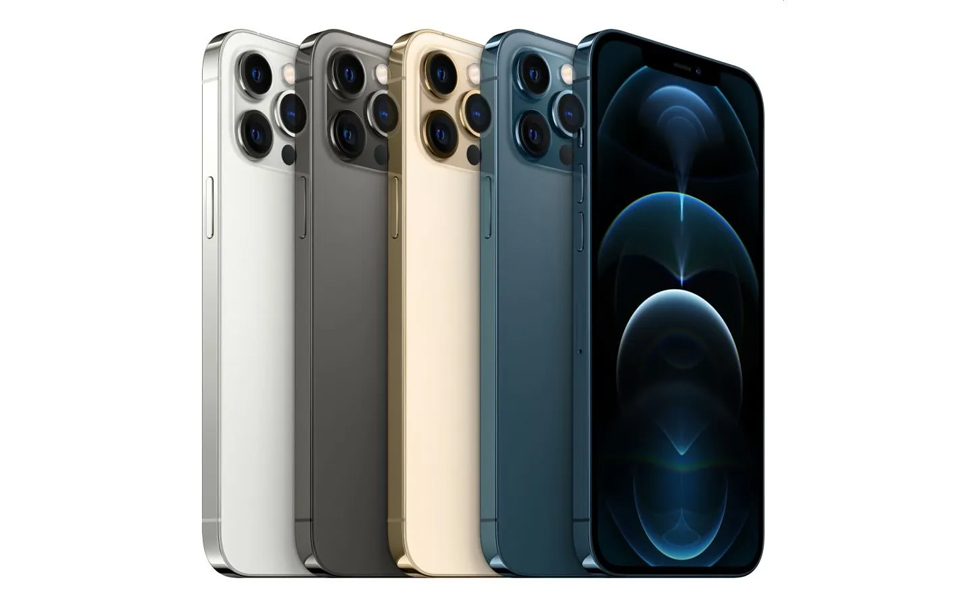
\includegraphics [width=0.3\textwidth]{iphone.jpg}}		
	
			\label{fig:fig2}
\end{center}	
\begin{center}		
			\subfigure[고민시]{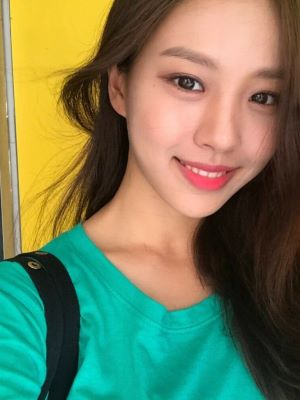
\includegraphics [width=0.2\textwidth]{gominsi.jpg}}
		\subfigure[고민시]
		{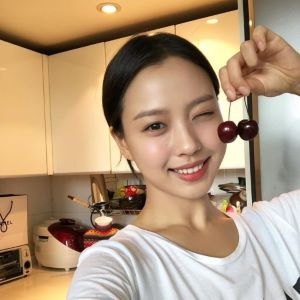
\includegraphics [width=0.2\textwidth]{gominsi2.jpg}}
\end{center}
\begin{center}		
	
			\subfigure[고민시]
			{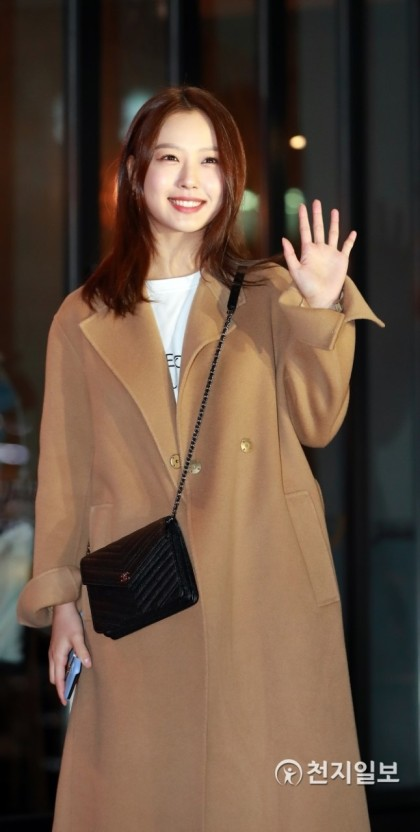
\includegraphics [width=0.2\textwidth]{gominsi3.jpg}}
		\subfigure[고민시]{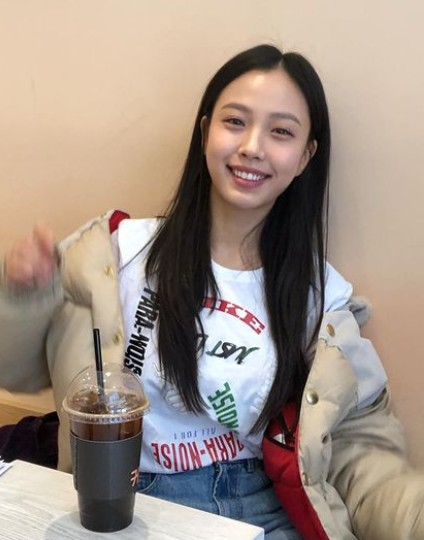
\includegraphics [width=0.2\textwidth]{gominsi4.jpg}}
			\caption{좋아하는 연예인}
		\label{fig:fig3}
\end{center}		
\end{figure}

\subsection{나를 나타내기}
저는 Figure ~\ref{fig:fig1}에서 보시는 것 처럼 홍익대학교에 재학 중인 3학년 컴퓨터공학과 학생 김영민입니다. 저는 컴퓨터 공학과 학생으로서 C언어, 자바, C++ 등등 여러 컴퓨터 언어들을 공부하고 있고 컴퓨터 구조, 운영체제 같은 컴퓨터의 전반적인 것들에 관해 더 배울 예정입니다. 홍익대학교의 유능한 교수님들로부터 많은 것들을 배우고 그림 Figure~\ref{fig:fig2}에서 보시다시피 저는 애플을 굉장히 좋아합니다. 핸드폰도 아이폰을 쓰고 있고 태블릿 PC도 아이패드를 쓰고 이어폰도 에어팟을 쓰고 있습니다.애플 제품들은 최적화가 굉장히 잘 되어 있고 소프트웨어와 하드웨어의 융합이 굉장히 조화롭게 이루어진 것 같습니다. 매년 신제품들이 나오는데, 매년 기능과 디자인이 혁신적인것 같습니다. 지금은 당연하게 느껴지지만, 스티브 잡스의 초기 스마트폰 출시 당시 사람들은 매우 놀랐고 우리는 전혀 예상하지 못한 세계가 왔습니다. 그래서 나중에 애플에서 일해보고 싶은 큰 욕망이 있습니다. 아직은 부족한 점들도 있지만 앞으로 공부하면서 채워 나갈 예정입니다.
\subsection{가장 좋아하는 연예인}

 저는 연예인 고민시를 좋아합니다. 예쁘고 연기도 잘하고 매력 있습니다. 그림 Figure~\ref{fig:fig3} 에서 보시는 것처럼 굉장히 단아하고 귀여워 보입니다. 옷도 잘 입고 비율도 좋습니다. 그리고 특히웃을때 매우 이쁩니다. 옛날에 영화 '마녀'에서 김다미의 친구 역할로 나왔을때는 잘 몰랐는데 좀 유명해지고 그때 알았습니다. 매우 예뻐서 인스타도 팔로우 해놨습니다. 저는 보지는 않았지만 넷플릭스 '스위트홈'에 고민시가 출연을 하였는데, 아주 연기가 뛰어나다고 들었습니다. 예쁘기 뿐만 아니라 연기도 잘 하는 것 같습니다. 앞으로 고민시가 영화나 드라마에 조금 더 자주 출연하는 모습을 보면 좋겠습니다. 

\end{document}
